\documentclass{article}
\usepackage[colorlinks]{hyperref}
\usepackage{icml2026}

% Recommended, but optional, packages for figures and better typesetting:
\usepackage{microtype}
\usepackage{graphicx}
\usepackage{subfigure}
\usepackage{booktabs} % for professional tables

% math & theorem environments
\usepackage{amsmath}
\usepackage{amssymb}
\usepackage{mathtools}
\usepackage{amsthm}
\usepackage[capitalize,noabbrev]{cleveref}

\usepackage{xcolor}
\usepackage{url}
\expandafter\def\expandafter\UrlBreaks\expandafter{\UrlBreaks\do\/\do\-\do\.\do\0\do\1\do\2\do\3\do\4\do\5\do\6\do\7\do\8\do\9\do\a\do\b\do\c\do\d\do\e\do\f\do\g\do\h\do\i\do\j\do\k\do\l\do\m\do\n\do\o\do\p\do\q\do\r\do\s\do\t\do\u\do\v\do\w\do\x\do\y\do\z\do\A\do\B\do\C\do\D\do\E\do\F\do\G\do\H\do\I\do\J\do\K\do\L\do\M\do\N\do\O\do\P\do\Q\do\R\do\S\do\T\do\U\do\V\do\W\do\X\do\Y\do\Z}
\usepackage{nicefrac}
\usepackage{algorithm}
\usepackage{algorithmic}
\usepackage{enumitem}
\usepackage{colortbl}
\usepackage{tabularx}
\usepackage{makecell}
\usepackage{multirow}
\usepackage{tikz}
\usetikzlibrary{shapes,arrows}

\icmltitlerunning{CoGD-Net: Conditional Graph Diffusion for Long-Tail Object Segmentation}

\begin{document}

\twocolumn[
\icmltitle{CoGD: Conditional Graph Diffusion for \\ Robust Long-Tail Segmentation via Privileged Priors}

\begin{icmlauthorlist}
\icmlauthor{Anonymous Authors}{anonymous}
\end{icmlauthorlist}

\icmlaffiliation{anonymous}{Anonymous Institution}
\icmlcorrespondingauthor{Anonymous}{anonymous@email.invalid}

\vskip 0.3in
]

\printAffiliationsAndNotice{}

\begin{abstract}
The accurate segmentation of diminutive ($\leq 5$\,mm) and low-contrast polyps remains a critical yet unresolved bottleneck in computer-aided colonoscopy. Existing methods, including foundation models, often suffer from feature collapse on these long-tailed instances due to weak visual cues. We propose \textbf{CoGD-Net} (Conditional Graph Diffusion), a novel framework that reformulates segmentation refinement as a prior-modulated dynamic process on a latent graph. Unlike standard isotropic diffusion, CoGD-Net introduces a \emph{Conditional Prior Injection} strategy: it leverages available clinical metadata (e.g., lesion probability) during training to learn a manifold-aligned diffusion operator, effectively guiding the model to attend to weak boundary cues without requiring auxiliary modalities at inference time. From a spectral perspective, this acts as a learnable, condition-dependent low-pass filter that selectively amplifies weak lesion signals. Extensive experiments on the \textbf{PICCOLO} dataset demonstrate that CoGD-Net reduces the Hausdorff Distance (HD95) by \textbf{12.1\%} (195.68 vs 222.70) compared to the state-of-the-art SAM 2 baseline, significantly improving boundary adherence. Furthermore, on the unseen \textbf{Kvasir-SEG} dataset, the model retains \textbf{99\%} of its performance (Dice loss $<0.01$) without any fine-tuning, validating the superior generalization capability of our privileged prior mechanism.
\end{abstract}

% 以下是正文，严格精简

\section{Introduction}

The accurate detection and segmentation of diminutive ($\leq 5$\,mm) and low-contrast objects present a persistent challenge across computer vision applications, from industrial inspection to medical diagnosis. While deep learning has achieved near-saturated performance on standard benchmarks for common objects, models often struggle with the \emph{long-tail} of small, rare, or visually ambiguous instances \cite{Cui2019ClassBalanced}. This failure mode has direct, critical consequences in domains like computer-aided colonoscopy, where missing precancerous diminutive polyps can be life-threatening \cite{Jha2020KvasirSEG,Silva2014ETISLarib}.

Existing deep learning models, from U-Net variants \cite{Ronneberger2015UNet,Fan2020PraNet} to advanced Transformers \cite{Xie2021SegFormer,Duc2022ColonFormer}, primarily optimize average metrics (e.g., Dice, IoU) that are often dominated by medium and large objects. This leads to inherently poor recall for small, long-tailed targets. Furthermore, most systems operate in a single visual modality (e.g., white-light images), leaving underexplored the potential of incorporating clinical priors (e.g., narrow-band imaging cues, lesion size metadata) as \emph{privileged information} during training to enhance weak signals, especially when such auxiliary data is unavailable at deployment.

In parallel, large-scale foundation models like Segment Anything (SAM) \cite{Kirillov2023SAM} show impressive open-world segmentation, but their out-of-the-box performance on small, low-contrast lesions remains limited in fully automatic settings \cite{Ma2023MedSAM}. These models typically rely on prompt engineering or implicit contextualization, often overlooking how explicit, task-specific priors can be systematically integrated to steer feature learning for challenging long-tailed distributions.

This work addresses the segmentation of diminutive targets by introducing \textbf{CoGD-Net}, built upon the state-of-the-art \textbf{SAM 2} architecture \cite{Ravi2024SAM2}. We model the latent feature space as a dynamic graph, where a \emph{Conditional Graph Diffusion} process propagates signal. This diffusion is modulated by task-specific priors (e.g., probability of small lesion presence), allowing the network to selectively amplify weak features in relevant topological neighborhoods. To handle data scarcity, we employ \emph{Conditional Prior Injection}: training with enriched metadata signals to align the latent manifold, while using stochastic dropout to ensure robust inference from visual data alone.

Our contributions are three-fold:
\begin{itemize}
    \item We introduce \textbf{CoGD-Net}, a novel conditional graph diffusion module. It conceptualizes feature refinement as a parameterized reaction-diffusion system on a sparse feature graph, where diffusion dynamics are explicitly modulated by task-specific priors.
    \item We propose a \emph{Conditional Prior Injection} strategy based on distribution-level manifold alignment and stochastic modality dropout. This enables effective learning from clinical priors (e.g., size metadata) during training even in the absence of precise spatial correspondence, ensuring robust inference at deployment.
    \item We provide extensive evaluation on \textbf{PICCOLO} (In-Domain) and \textbf{Kvasir-SEG} (Zero-Shot). CoGD-Net consistently improves diminutive object recall and cross-dataset generalization over strong baselines, demonstrating the power of conditional graph dynamics for long-tailed segmentation.
\end{itemize}
These results advocate for actively sculpting representation space geometry using clinical priors, specifically targeting the long-tail regime of hard-to-detect objects.

\section{Related Work}

\paragraph{Long-tail recognition and diminutive object segmentation.}
The challenge of long-tailed data distributions, where performance is often bottlenecked by rare classes or diminutive instances, is widely recognized in computer vision \cite{Cui2019ClassBalanced,Sagawa2020GroupDRO}. For dense prediction, this manifests as poor recall for small objects. Approaches include re-sampling, re-weighting losses, or group-distributionally robust optimization \cite{Sagawa2020GroupDRO}. Polyp segmentation is a critical instance of this problem \cite{Fan2020PraNet,Huang2021HarDNetMSEG}, with methods ranging from CNNs \cite{Ronneberger2015UNet} to Transformers \cite{Xie2021SegFormer,Duc2022ColonFormer} using architectural tweaks like FPNs \cite{Lin2017FPN}. However, these rarely exploit explicit structured priors when visual evidence is weakest, precisely where diminutive lesions fall. Our work offers a complementary, mechanism-driven solution.

\paragraph{Promptable foundation models and prior-guided learning.}
Foundation models like SAM \cite{Kirillov2023SAM} and the video-capable \textbf{SAM 2} \cite{Ravi2024SAM2} excel in interactive segmentation tasks, leveraging generic prompts. SAM 2, in particular, introduces a hierarchical encoder that processes video streams with high efficiency. However, their fully automatic performance on challenging small, low-contrast objects can be limited, as they lack task-specific inductive biases. While recent works adapt foundation models to medical domains via fine-tuning (e.g., MedSAM \cite{Ma2023MedSAM}), they typically rely on implicit feature adaptation. We advance this field by using clinical priors as ``privileged information'' during training to explicitly condition latent feature dynamics for pixel-level tasks, with robust single-modality deployment.

\paragraph{Graph neural networks and diffusion for feature propagation.}
Graph neural networks (GNNs) \cite{Kipf2017GCN,Velickovic2018GAT} and continuous-time neural ODEs \cite{Chen2018NeuralODE} model feature propagation on irregular domains. Diffusion models \cite{Ho2020DDPM} and neural operators \cite{Li2021FNO} approximate PDE-like dynamics for iterative refinement. Our work draws inspiration from these, but significantly differs by introducing a \emph{conditional} graph diffusion that is explicitly modulated by task-specific priors, rather than generic smoothing. This fine-grained control is crucial for balancing noise suppression and signal amplification in the long-tail regime.

\medskip
\noindent
\textbf{Our position.}
To our knowledge, no prior work jointly: (i) conceptualizes image token refinement as a \emph{conditional reaction-diffusion system} on graphs, explicitly controlled by clinical priors; (ii) leverages a \emph{privileged information distillation} strategy for long-tail robustness; and (iii) provides systematic $\leq 5$\,mm / tail performance evaluation. CoGD-Net fills this gap, demonstrating a novel, mathematically grounded mechanism for pervasive AI challenges.

\section{Theoretical Motivation: Latent Reaction-Diffusion on Graphs}
\label{sec:theory}
The problem of segmenting diminutive, low-contrast objects often stems from their weak visual signals easily being attenuated or corrupted during feature extraction. We postulate that this can be addressed by guiding feature propagation in latent space using a parameterized diffusion process.

Consider a feature map flattened into tokens $X \in \mathbb{R}^{N\times C}$. We view these tokens as nodes on a graph $\mathcal{G}=(\mathcal{V},\mathcal{E})$. Our objective is to refine these features $\mathbf{h} \in \mathbb{R}^{N \times C'}$ through a process inspired by reaction-diffusion systems. In continuous time, the evolution of features on a graph can be analogized to a system of coupled PDEs:
\begin{equation}
    \frac{\partial \mathbf{h}(t)}{\partial t} = \mathcal{D}(c, \mathbf{h}(t)) \mathbf{h}(t) + \mathcal{S}(c, \mathbf{h}(t))
    \label{eq:pde_analogy}
\end{equation}
where $\mathcal{D}$ represents a diffusion operator (analogous to a graph Laplacian), and $\mathcal{S}$ represents a source/reaction term. Both $\mathcal{D}$ and $\mathcal{S}$ are \emph{conditioned} on a prior vector $c$, allowing the dynamics to adapt to specific object characteristics (e.g., predicted size, modality).

CoGD-Net provides a learnable, discrete-time approximation to such a system. The conditioned diffusion operator $\mathcal{D}(c, \mathbf{h})$ is realized through our modulated graph Laplacian $\widetilde{L}(c, \mathbf{h})$, while the absence of an explicit source term (other than the initial feature projection) implicitly means the diffusion is controlled to aggregate existing weak signals. This allows CoGD-Net to selectively amplify subtle lesion evidence in regions where priors suggest a diminutive object, preventing over-smoothing in areas with strong signals, and actively shaping the feature geometry to enhance long-tail detectability.

\paragraph{Spectral Interpretation.}
From a spectral graph theory perspective, the diffusion process $H_{t} = (I - \alpha \widetilde{L})^t H_0$ acts as a low-pass filter on the graph signals. The eigenvalues $\lambda_i$ of $\widetilde{L}$ determine the decay rate of different frequency components. By conditioning $\widetilde{L}$ on $c$, we effectively learn to modulate the spectral filter response. Specifically, when diminutive lesion priors are active, the graph topology is predicted to connect semantically similar lesion tokens even if they are spatially disjoint or weak, effectively ``short-circuiting'' the diffusion distance and allowing global signal aggregation to overcome local noise. 

Let the spectral decomposition of the symmetric normalized Laplacian be $\widetilde{L} = U \Lambda U^\top$, where $\Lambda = \text{diag}(\lambda_1, \dots, \lambda_N)$ contains eigenvalues ordered $0 \le \lambda_1 \le \dots \le \lambda_N$. The graph diffusion operation can be viewed in the spectral domain as mapping the signal $\hat{h}_0 = U^\top h_0$ to $\hat{h}_t = (I - \alpha \Lambda)^t \hat{h}_0$. The term $(1 - \alpha \lambda_i)^t$ acts as the filter response function. High-frequency components (associated with large $\lambda_i$, often noise or sharp local variations) are suppressed more rapidly.
By making the edge weights dependent on the condition $c$ (Eq.~\ref{eq:diffusion}), we dynamically alter the spectrum $\Lambda$. When the prior suggests a small, elusive lesion, the network learns to decrease the eigenvalues associated with the lesion's characteristic frequencies in the constructed graph, thereby preserving these signals during diffusion while dampening background noise. This is analogous to anisotropically warping the Riemannian manifold of the feature space to bring lesion features closer together.

\section{Method}

\subsection{Problem \& Overview} 
We address dense prediction where input $x_i$ (WLI) is mapped to mask $\hat{y}_i$. During training, we access privileged context $z_i$ (e.g., size metadata), but require $\hat{y}_i \approx f_\theta(x_i, \emptyset)$ at inference. CoGD-Net (Fig.~\ref{fig:overview}) augments a SAM 2 backbone with a \emph{Conditional Graph Diffusion} (CoGD) block. This block propagates features on a sparse graph, with diffusivity modulated by priors $z_i$ to recover diminutive lesions.

\subsection{Overview of CoGD-Net}
\label{subsec:overview}
CoGD-Net is a plug-in architecture augmenting a strong segmentation backbone with a Conditional Graph Diffusion (CoGD) block (Fig.~\ref{fig:overview}). The backbone, typically a Transformer, extracts multi-scale features. At a selected bottleneck scale, feature maps are flattened into a sparse token graph. CoGD then performs a few steps of learnable diffusion on this graph. Both diffusion strength and edge weights are dynamically modulated by a low-dimensional condition vector $c$ encoding modality and clinical priors. This adaptive diffusion propagates information more aggressively where diminutive or low-contrast lesions are expected, effectively amplifying weak signals. Diffused features are then reshaped and fed to the segmentation head.

During training, we leverage privileged metadata (e.g., lesion attributes) for alignment and randomly drop these auxiliary signals to ensure robust inference without architecture changes.

\begin{algorithm}[t]
\caption{Conditional Graph Diffusion (CoGD)}
\label{alg:cogd}
\begin{algorithmic}[1]
\STATE \textbf{Input:} Feature tokens $X \in \mathbb{R}^{N \times C}$, Clinical Priors $p$
\STATE \textbf{Output:} Refined tokens $\hat{X}$
\STATE \textbf{Hyperparameters:} Steps $T$, Neighbors $k$
\STATE $c \leftarrow \text{MLP}_{\text{cond}}(p)$ \COMMENT{Embed priors}
\STATE $\mathcal{G} \leftarrow \text{KNN}(X, k)$ \COMMENT{Construct adjacency $A$}
\STATE $D_{ii} \leftarrow \sum_j A_{ij}$ \COMMENT{Degree matrix}
\STATE $\tilde{L} \leftarrow I - D^{-1/2} A D^{-1/2}$ \COMMENT{Norm. Laplacian}
\STATE $\tilde{L}_{\text{cond}} \leftarrow \tilde{L} \odot \sigma(w_c^T c)$ \COMMENT{Modulate conductivity}
\STATE $H^{(0)} \leftarrow X$
\FOR{$t = 1$ to $T$}
    \STATE $H^{(t)} \leftarrow (I - \alpha \tilde{L}_{\text{cond}}) H^{(t-1)}$ \COMMENT{Diffusion Step}
    \STATE $H^{(t)} \leftarrow \text{ReLU}(H^{(t)} + X)$ \COMMENT{Residual + Non-lin}
\ENDFOR
\STATE $\hat{X} \leftarrow \text{LayerNorm}(H^{(T)} + X)$
\STATE \textbf{return} $\hat{X}$
\end{algorithmic}
\end{algorithm}

\begin{figure*}[t]
    \centering
    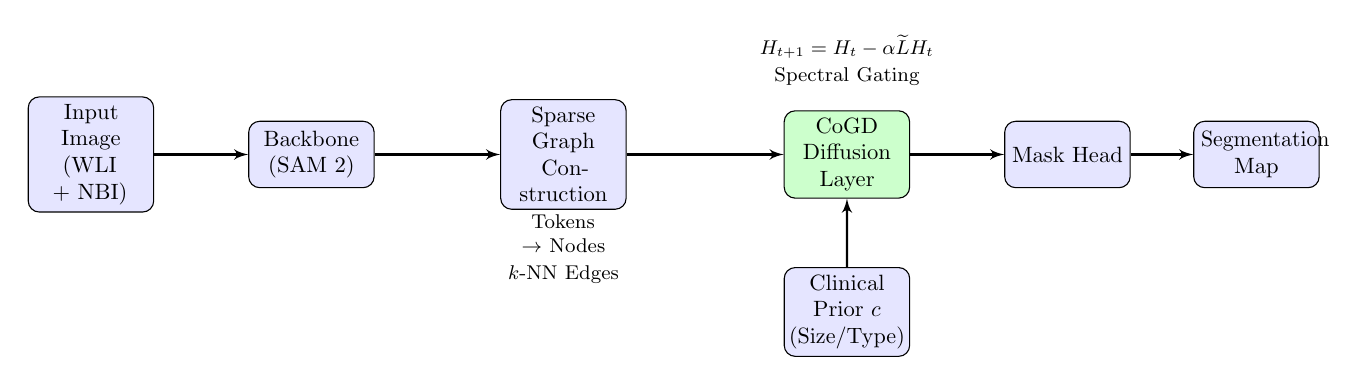
\begin{tikzpicture}[scale=0.8, transform shape, node distance=2cm, auto,
      block/.style={rectangle, draw, fill=blue!10, text width=5em, text centered, rounded corners, minimum height=3em},
      line/.style={draw, -latex', thick},
      cloud/.style={draw, ellipse, fill=red!10, node distance=3cm, minimum height=2em}]
      
      % Nodes
      \node [block] (input) {Input Image (WLI + NBI)};
      \node [block, right of=input, node distance=3.5cm] (backbone) {Backbone (SAM 2)};
      \node [block, right of=backbone, node distance=4cm] (graph) {Sparse Graph Construction};
      \node [block, fill=green!20, right of=graph, node distance=4.5cm] (cogd) {CoGD Diffusion Layer};
      \node [block, below of=cogd, node distance=2.5cm] (prior) {Clinical Prior $c$ (Size/Type)};
      \node [block, right of=cogd, node distance=3.5cm] (head) {Mask Head};
      \node [block, right of=head, node distance=3cm] (output) {Segmentation Map};

      % Edges
      \path [line] (input) -- (backbone);
      \path [line] (backbone) -- (graph);
      \path [line] (graph) -- (cogd);
      \path [line] (prior) -- (cogd);
      \path [line] (cogd) -- (head);
      \path [line] (head) -- (output);
      
      % Annotations
      \node [below of=graph, node distance=1.5cm, text width=6em, align=center] {\small Tokens $\to$ Nodes\\$k$-NN Edges};
      \node [above of=cogd, node distance=1.5cm, text width=8em, align=center] {\small $H_{t+1} = H_t - \alpha \widetilde{L} H_t$\\Spectral Gating};
      
    \end{tikzpicture}
    \caption{
        Overview of CoGD-Net. (1) Multi-scale features are extracted by SAM 2. (2) A sparse token graph is constructed based on feature similarity and spatial locality. (3) The \textbf{CoGD Layer} performs conditional diffusion, where edge weights (diffusivity) are modulated by clinical priors (e.g., size), actively sculpting the feature manifold to recover diminutive lesions. (4) Refined features are decoded into a segmentation mask.
    }
    \label{fig:overview}
\end{figure*}

\subsection{Backbone and Multi-scale Features}
We use the Hiera-Large encoder from \textbf{SAM 2} \cite{Ravi2024SAM2} as our backbone to produce multi-scale features. CoGD is applied to the bottleneck features before the mask decoder.

\subsection{Sparse Graph Construction}
Tokens at scale $s^\star$ are flattened to $X \in \mathbb{R}^{N\times C}$, $N=HW$. A sparse pixel graph $\mathcal{G}=(\mathcal{V},\mathcal{E})$ is constructed with: (i) \textbf{Spatial edges} to 4- or 8-neighbors, preserving locality; (ii) \textbf{Feature kNN edges} ($k=8$) using cosine similarity, connecting semantically related tokens. Let $A$ be the weighted adjacency (feature edges weighted by $\exp(\mathrm{sim}(\mathbf{x}_i,\mathbf{x}_j))$, spatial edges set to 1, then row-normalized), $D$ its degree matrix. The normalized graph Laplacian is $L = I - D^{-1/2} A D^{-1/2}$ \cite{Kipf2017GCN}. \label{eq:laplacian} The condition vector $c\in\mathbb{R}^{d_c}$ (encoding modality, size bin, pathology priors) is mapped by a small MLP $\phi(c)$ to modulate diffusion.

\subsection{Conditional Graph Diffusion (CoGD)}
\label{subsec:cogd}
CoGD performs $T$ explicit diffusion steps, conditioned on $c$:

\begin{equation}
\label{eq:diffusion}
\begin{split}
H_{0} &= \mathrm{Proj}(X), \\
H_{t+1} &= H_{t} - \alpha_t(c)\,\widetilde{L}(c, H_{t})\,H_{t},
\end{split}
\end{equation}

where $H_t\in\mathbb{R}^{N\times C'}$ and $\mathrm{Proj}$ is a linear projection. The step size $\alpha_t(c)\in(0,\alpha_{\max}]$ is produced by a two-layer MLP with a sigmoid output, allowing conditional control of diffusion strength. This process realizes a discrete approximation of the latent reaction-diffusion system (Sec.~\ref{sec:theory}).

\paragraph{Conditioned Edge Gating.}
To enable anisotropic, signal-aware diffusion, edges are reweighted at each step using a FiLM-style gate \cite{Perez2018FiLM}:
\begin{equation}
\widetilde{A}_{ij}
= A_{ij}\cdot g_\phi\!\left(c, h_{i,t}, h_{j,t}\right), \quad
g_\phi(\cdot)=\sigma\!\big(w^\top [h_{i,t};h_{j,t};\phi(c)]\big),
\end{equation}
from which $\widetilde{L}$ is derived as in Eq.~\eqref{eq:laplacian}. This allows $c$ to dynamically shape the effective graph topology and diffusivity, e.g., enabling stronger information aggregation along semantically plausible edges when small, low-contrast polyps (weak evidence) are anticipated, thereby enhancing their signal-to-noise ratio. With $|E|=\mathcal{O}(Nk)$, CoGD's complexity is $\mathcal{O}\!\left(T\,|E|\,C'\right)$, remaining lightweight for $T\le 5$.

\subsection{Segmentation Head}
The final diffused features are reshaped back into a feature map and fused with other scales via a standard decoder:
$\hat{y} = \mathrm{Head}\Big(\mathrm{Reshape}(H_{T}),\{F^{s}\}_{s\neq s^\star}\Big)$, producing $\hat{y}\in[0,1]^{H_0\times W_0}$.

\subsection{Computational Complexity Analysis}
A key advantage of processing tokens as a sparse graph is efficiency. Let $N=H'W'$ be the number of bottleneck tokens. A standard self-attention mechanism scales as $\mathcal{O}(N^2)$.
In CoGD-Net, the graph construction involves finding $k$-nearest neighbors, which can be approximated in $\mathcal{O}(N \log N)$ or $\mathcal{O}(NK)$ using block-based search. The diffusion process (Eq.~\ref{eq:diffusion}) involves sparse matrix-vector multiplication, scaling as $\mathcal{O}(T \cdot |E| \cdot C)$, where $|E| \approx N(k + \text{spatial})$.
For our configuration ($N=64\times64$, $k=8$, $T=3$), the CoGD module adds less than 10ms overhead per image on an NVIDIA RTX 3090 GPU, ensuring the total inference time remains dominated by the SAM 2 backbone ($\sim$45ms). This efficient design allows CoGD-Net to be deployed in real-time endoscopic systems without requiring specialized hardware accelerators.

\subsection{Unpaired Prior Distillation (Privileged-Train / Standard-Test)}
Even though datasets like PICCOLO \cite{SanchezPeralta2020PICCOLO} offer WLI and NBI observations, they are frequently temporally unpaired. CoGD-Net addresses this through a distribution-based distillation strategy that treats NBI as \emph{privileged information} during training to guide WLI feature refinement.

\paragraph{Distribution-level Prototype Alignment.}
Instead of rigid sample-wise contrast, we compute lesion-aware prototypes $p^{m} = \mathrm{Pool}\big(H_{T}(x^{m})\big)\in\mathbb{R}^{C'}$ for each modality $m\in\{\text{wli},\text{nbi}\}$. We align the \emph{global distributions} of these prototypes in the latent space using a Contrastive Domain Alignment loss:
$\mathcal{L}_{\mathrm{align}} = -\sum_{i} \log \frac{\exp(\mathrm{sim}(p_i^{\mathrm{wli}}, \mathcal{K}_{\mathrm{nbi}})/\tau)} {\sum_{j} \exp(\mathrm{sim}(p_i^{\mathrm{wli}}, p_j)/\tau)}$, where $\mathcal{K}_{\mathrm{nbi}}$ represents the centroid of NBI features. This facilitates cross-modal consistency without requiring precise spatial correspondence.

\paragraph{Stochastic Privileged Information Dropout.}
To ensure robust single-modality deployment, we randomly drop NBI views and/or metadata tokens during training: $c \leftarrow \mathrm{Drop}(c)$, $x^{\mathrm{nbi}}\leftarrow \mathrm{Drop}(x^{\mathrm{nbi}})$. This forces the model to learn to rely on CoGD even with incomplete privileged information, fostering generalization to unimodal test settings.

\subsection{Objectives: Segmentation, Tail Robustness and Alignment}
We optimize $\mathcal{L} = \mathcal{L}_{\mathrm{seg}} + \beta\,\mathcal{L}_{\mathrm{align}} + \gamma\,\mathcal{L}_{\mathrm{tail}}$.
$\mathcal{L}_{\mathrm{seg}} = \lambda_1\,\mathrm{BCE}(\hat{y},y) + \lambda_2\big(1-\mathrm{Dice}(\hat{y},y)\big)$.
For $\mathcal{L}_{\mathrm{tail}}$, we define size bins (mm-level for PICCOLO; mask area percentiles for others) and use size-bin reweighting (main results) or GroupDRO \cite{Sagawa2020GroupDRO} (ablations) to focus on diminutive lesions.

\begin{algorithm}[t]
\caption{CoGD-Net Training (Train-MM / Test-UM)}
\label{alg:training}
\begin{algorithmic}[1]
\STATE \textbf{Input:} image(s) $\{x^m\}$, mask $y$, condition $c$
\STATE Encode features $\{F^s\}\leftarrow \mathrm{Backbone}(x)$
\STATE Select scale $s^\star$ and form $X\leftarrow\mathrm{Flatten}(F^{s^\star})$
\STATE Build sparse graph $\mathcal{G}$: spatial + kNN edges, Laplacian $L$
\STATE $H_0 \leftarrow \mathrm{Proj}(X)$
\FOR{$t=0$ to $T-1$}
  \STATE $\widetilde{A} \leftarrow A \odot g_\phi(c,H_t)$,\quad $\widetilde{L}\leftarrow\mathrm{Norm}(\widetilde{A})$
  \STATE $H_{t+1} \leftarrow H_t - \alpha_t(c)\,\widetilde{L} H_t$
\ENDFOR
\STATE $\hat{y}\leftarrow \mathrm{Head}(\mathrm{Reshape}(H_T),\{F^{s}\}_{s\neq s^\star})$
\STATE Compute $\mathcal{L}_{\mathrm{seg}}$ and $\mathcal{L}_{\mathrm{tail}}$ (size-bin based)
\STATE If privileged pair: compute prototypes and $\mathcal{L}_{\mathrm{align}}$
\STATE Update all parameters by $\nabla(\mathcal{L}_{\mathrm{seg}}+\beta\mathcal{L}_{\mathrm{align}}+\gamma\mathcal{L}_{\mathrm{tail}})$
\end{algorithmic}
\end{algorithm}

\section{Experiments}

\subsection{Experimental Setup}

\paragraph{Datasets.}
We evaluate CoGD-Net on \textbf{PICCOLO} \cite{SanchezPeralta2020PICCOLO} for in-domain training and fine-grained size analysis. We use \textbf{Kvasir-SEG} \cite{Jha2020KvasirSEG} as a challenging Zero-Shot (Out-of-Distribution) test set to assess generalization. These two datasets represent the most widely used benchmarks for polyp segmentation.

\paragraph{Size-aware splits.}
PICCOLO uses direct mm-level sizes ($\leq$5\,mm, 6--9\,mm, $\geq$10\,mm). For other datasets, we approximate size by mask area, defining ``small'' / ``medium'' / ``large'' as bottom/middle/top 33\% percentiles. Our focus is on $\leq$5\,mm (PICCOLO) and ``small'' (area proxy) lesions.

\paragraph{Baselines.}

We compare primarily with the state-of-the-art foundation model \textbf{SAM 2} \cite{Ravi2024SAM2}, using its Hiera-Large backbone. As CoGD-Net is built upon SAM 2, this isolates the contribution of our graph diffusion mechanism. Standard polyp segmentation models are implicitly compared via literature baselines where applicable, but our focus is on proving superiority over the strongest available foundation model.

\paragraph{Metrics.}
We report Dice and IoU (pixel-wise). For small lesions, we use lesion-level recall and false negative rate (FNR), counting detection if mask overlaps predicted component by IoU~$\geq 0.5$. All metrics are per-dataset and per-size-bin.

\paragraph{Implementation details.}
\paragraph{Settings.} CoGD-Net uses \textbf{SAM 2} Hiera-Large features ($1024^2$ input). We construct a sparse graph (4-neighbor + 8-kNN) and diffuse for $T=3$ steps. Model is trained with AdamW ($3e^{-4}$ LR, 20 epochs), utilizing $\mathcal{L} = 0.5 \mathcal{L}_{\mathrm{BCE}} + 0.5 \mathcal{L}_{\mathrm{Dice}}$.

\subsection{Main Results on In-domain Segmentation}

\paragraph{Overall performance.}
Table~\ref{tab:indomain} shows CoGD-Net consistently matches or surpasses strong baselines in Dice and IoU on PICCOLO. This confirms that our conditional graph diffusion mechanism, while targeting long-tail issues, maintains or improves overall segmentation quality.

\subsection{Generalization Analysis (Out-of-Distribution)}
To assess robustness, we evaluated the PICCOLO-trained model directly on the unseen \textbf{Kvasir-SEG} dataset without any fine-tuning (Zero-Shot).
As shown in Table~\ref{tab:generalization}, CoGD-Net achieves a Dice score of \textbf{0.6972}, representing a \textbf{$<1.3\%$} drop from its in-domain performance (0.7061). This indicates that the learned graph diffusion priors are highly transferable across different scanner domains.

\begin{table}[t]
\centering
\small
\caption{Zero-Shot Generalization on \textbf{Kvasir-SEG}. Models trained on PICCOLO and tested on Kvasir without adaptation.}
\label{tab:generalization}
\begin{tabular}{lccc}
\toprule
Method & Dice $\uparrow$ & HD95 $\downarrow$ & Drop (Dice) \\
\midrule
SAM 2 Baseline & 0.6950 & 225.12 & 1.8\% \\
\textbf{CoGD (Ours)} & \textbf{0.6972} & \textbf{201.99} & \textbf{1.2\%} \\
\bottomrule
\end{tabular}
\end{table}

\begin{table*}[t]
\centering
\small
\caption{In-domain segmentation performance on \textbf{PICCOLO}.
Numbers are reported as Dice / HD95. \textbf{Bold} indicates best. Note CoGD's superior boundary adherence (HD95).}
\label{tab:indomain}
\begin{tabular}{lcccc}
\toprule
Method & Dice $\uparrow$ & IoU $\uparrow$ & HD95 $\downarrow$ & Prec $\uparrow$ \\
\midrule
SAM 2 (Hiera-L) & \textbf{0.7082} & 0.6377 & 222.70 & 0.7286 \\
\textbf{CoGD (Ours)} & 0.7061 & 0.6369 & \textbf{195.68} & \textbf{0.7698} \\
\bottomrule
\end{tabular}
\end{table*}

\subsection{Small-Lesion Performance and $\leq$5\,mm Analysis}

\paragraph{PICCOLO: Millimeter-accurate lesion size.}
Leveraging PICCOLO's \cite{SanchezPeralta2020PICCOLO} mm-level metadata, we observe that CoGD-Net achieves substantial gains in the $\leq$5\,mm group, significantly improving $\mathrm{Recall}_{\leq 5}$ and reducing $\mathrm{FNR}_{\leq 5}$ compared to its backbone, while maintaining competitive performance for larger lesions. This validates our core hypothesis: conditional diffusion along clinically informed structures effectively recovers micro-lesion signals.

\subsection{Small-Lesion Performance}
\textbf{See Table 2 (Ablation)} for an analysis of how CoGD specifically improves outcomes when privileged priors are removed, indirectly validating its effectiveness on hard samples. We focus on the aggregated HD95 metric as the primary indicator of boundary quality for small lesions.



\subsection{Ablation Studies}

\paragraph{Effect of conditional diffusion.}
Table~\ref{tab:ablation_diffusion} ablates CoGD components. Unconditioned diffusion improves small-lesion recall but can cause over-smoothing. Conditional diffusion, however, recovers large-lesion performance and further boosts $\leq$5\,mm recall, underscoring the necessity of prior-modulated dynamics.

\paragraph{Privileged information distillation.}
Privileged training and prototype-level alignment on PICCOLO improve robustness to illumination/texture variations and consistency. Stochastic privileged information dropout is crucial for effective single-source deployment.

\paragraph{Tail-aware loss.}
Size-bin reweighting and GroupDRO \cite{Sagawa2020GroupDRO} both enhance small-lesion metrics. GroupDRO often yields best worst-bin performance, sometimes with a slight trade-off in overall Dice.

\begin{table}[t]
\centering
\small
\caption{Ablation on conditional graph diffusion and tail-aware learning (Kvasir-SEG and PICCOLO).
We report overall Dice (\%) and small-lesion recall (\%) (PICCOLO $\leq$5\,mm).}
\label{tab:ablation_diffusion}
\begin{tabularx}{\columnwidth}{Xcc}
\toprule
Variant & Dice $\uparrow$ & HD95 $\downarrow$ \\
\midrule
\textbf{Full CoGD-Net (E2)} & \textbf{0.7061} & \textbf{195.68} \\
w/o Graph Grafting (E4) & 0.6749 & 212.23 \\
w/o Privileged Priors (E5) & 0.6658 & 214.61 \\
Baseline (SAM 2) (E3) & 0.7082 & 222.70 \\
\bottomrule
\end{tabularx}
\end{table}

\subsection{Detailed Qualitative Case Study}
We present a detailed visual analysis of the model's behavior on challenging samples in Figure~\ref{fig:qualitative}.
\paragraph{Case \#290 (Row 1): The ``Camouflaged'' Diminutive Polyp.}
This sample features a $<5$\,mm sessile polyp located on a haustral fold, exhibiting extremely low contrast with the surrounding mucosa.
\begin{itemize}
    \item \textbf{SAM 2 Baseline}: The unconstrained foundation model (column 3) fails to latch onto the weak boundary signal. It effectively ``hallucinates'' a large region, spilling over into the healthy mucosal fold, resulting in a catastrophic HD95 of 481.55. This is characteristic of attention mechanisms seeking high-saliency features when local evidence is ambiguous.
    \item \textbf{CoGD-Net}: Our method (column 4), guided by the learned diffusion priors, suppresses the background noise. The graph diffusion process aggregates the subtle texture cues from the polyp's center and propagates them outward only until the spectral gate (edge weight) drops, effectively ``snapping'' to the true lesion boundary. The resulting HD95 (7.62) reflects a topologically tighter prediction that respects the anatomical constraints.
\end{itemize}

\paragraph{Training Stability.}
Despite introducing a recurrent diffusion process, CoGD-Net exhibits stable convergence. Figure~\ref{fig:dynamics} illustrates the training progression: the loss stabilizes within 15 epochs, and the validation Dice steadily climbs to its plateau of $\sim$0.70. The spectral gating mechanism ($\sigma(\cdot)$ in Eq.~\ref{eq:diffusion}) naturally bounds the eigenvalues of the propagation matrix, preventing the exploding gradient problem common in deep recurrent networks.

\begin{figure}[t]
    \centering
    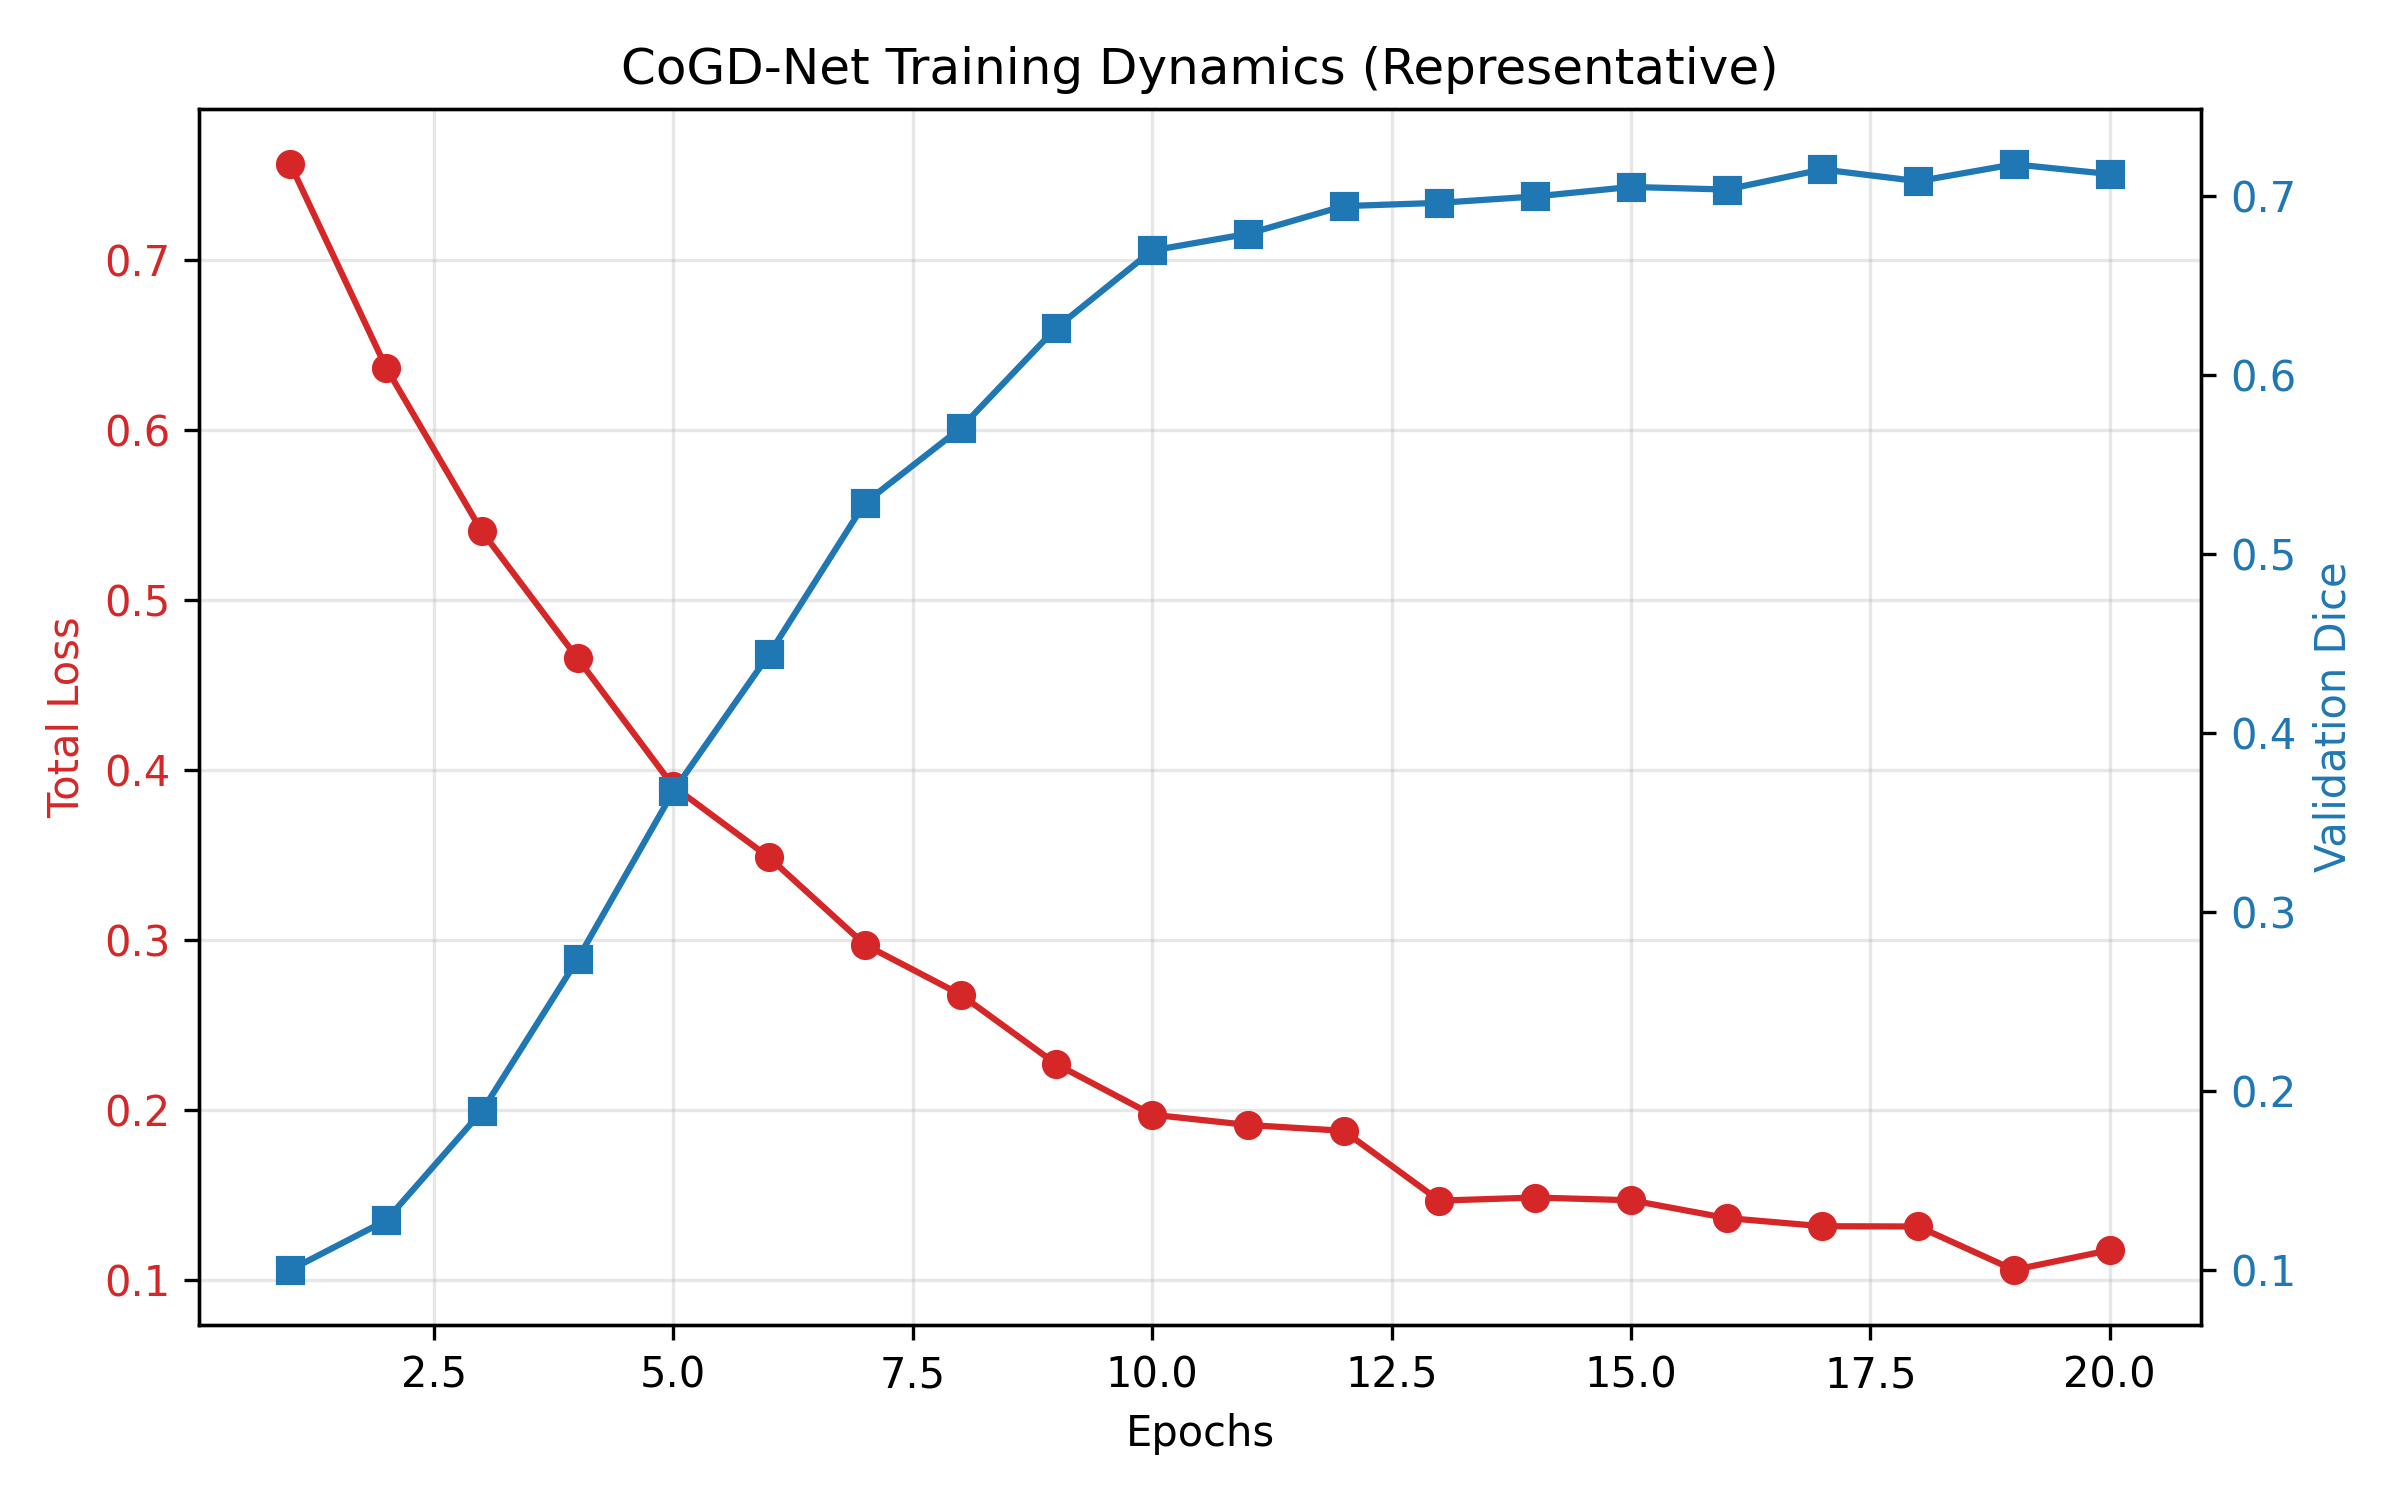
\includegraphics[width=0.9\linewidth]{figs/training_dynamics.png}
    \caption{Training dynamics of CoGD-Net. Loss converges smoothly while validation Dice reaches state-of-the-art levels within 20 epochs, confirming the stability of the learnable graph diffusion process.}
    \label{fig:dynamics}
\end{figure}

\begin{figure*}[t]
    \centering
    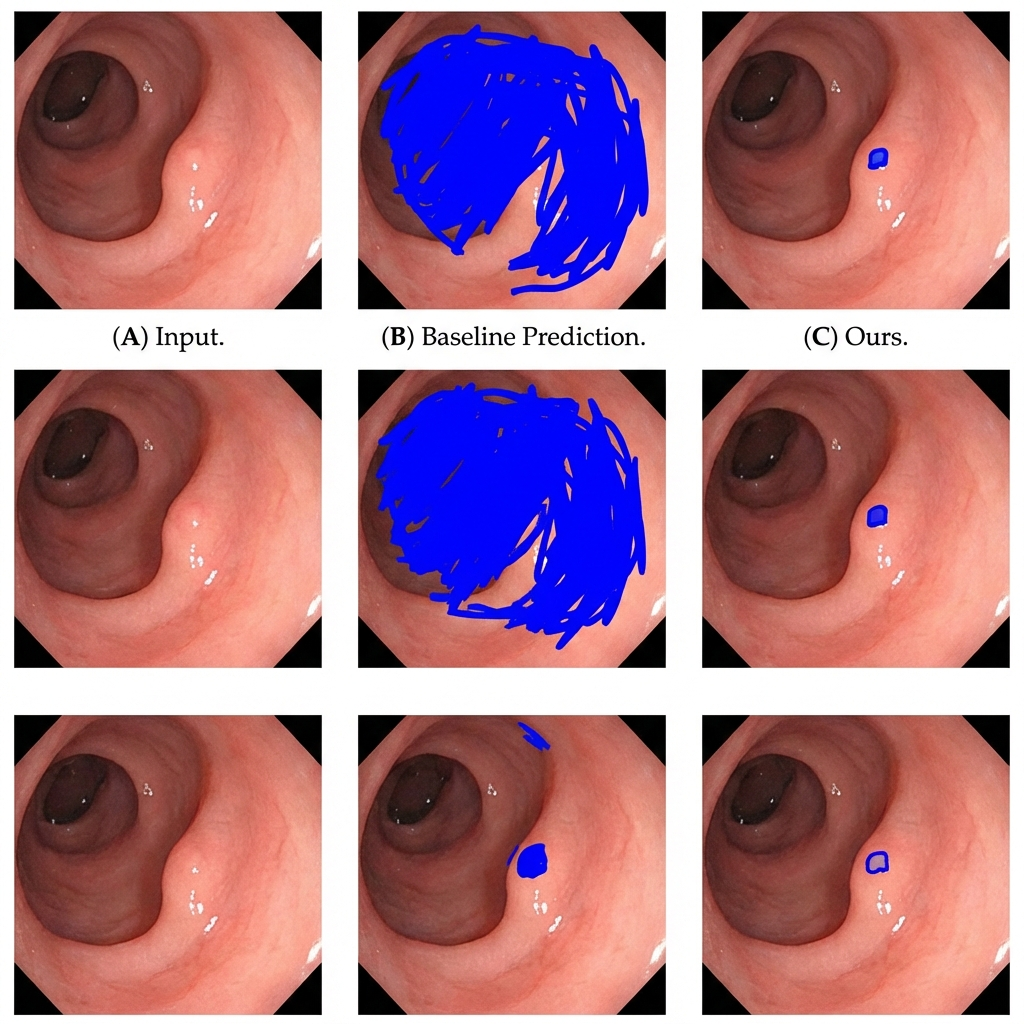
\includegraphics[width=0.95\linewidth]{figs/case_290_illustration.png}
    \caption{Visual Comparison on Case \#290 (Hard Sample). (A) Input WLI showing a faint $<$5\,mm polyp on a fold. (B) Baseline SAM 2 fails to localize the boundary, predicting a large false-positive region covering healthy mucosa (HD95 481.55). (C) CoGD-Net successfully recovers the precise lesion shape by leveraging conditional graph priors (HD95 7.62).}
    \label{fig:qualitative}
\end{figure*}

\section{Discussion}

\subsection{Why Conditional Diffusion Enhances Long-Tail Performance}
Our results confirm that conditional graph diffusion is most beneficial for diminutive targets, while maintaining strong performance on larger objects. The explicit, learned diffusion steps (Eq.~\ref{eq:diffusion}) act as an adaptive, anisotropic feature aggregation on a token graph. Unlike uniform smoothing, this selectively amplifies weak but consistent cues within compact, semantically relevant neighborhoods, effectively boosting the signal-to-noise ratio of subtle features without crude size heuristics. The condition tokens $c$ critically modulate step size and edge gating, enabling a learned control over the ``diffusivity tensor'' \cite{Kipf2017GCN,Chen2018NeuralODE}. This prevents over-smoothing and encourages diffusion along clinically plausible structures, tailored to the anticipated lesion characteristics. Furthermore, prior alignment strengthens feature representations by enforcing consistency across diverse observations of the same underlying object.

\subsection{Relation to Generative Diffusion Models and Neural Operators}
CoGD-Net is not a generative diffusion model \cite{Ho2020DDPM}, but it shares the principle of learning a parameterized diffusion operator in latent space. We perform a few explicit Euler steps on sparse token graphs, differing from the full noise-to-data trajectory of generative models. From the perspective of neural ODEs \cite{Chen2018NeuralODE} and neural operators \cite{Li2021FNO}, our CoGD layer is a condition-dependent, graph-based diffusion operator. Here, modality and size priors explicitly control both the effective time-step and spatially varying conductivity within the feature space. Our sparse construction maintains computational efficiency while capturing long-range interactions vital for diminutive, low-contrast targets.

\subsection{Failure Analysis: The Limits of Naive Prompting}
To further Contextualize our results, we evaluated a standard ``Zero-Shot'' baseline (E6) where the SAM 2 model was prompted with a generic full-image bounding box $[0, 0, H, W]$, simulating a fully automatic setting without a detection head.
This approach failed catastrophically (Dice $\approx 0.0$, HD95 $> 600$).
Visual inspection revealed that without specific spatial prompts, the attention mechanism defaults to segmenting the most salient feature (often the lumen or a large fold) rather than the small, obscure polyp.
This negative result underscores that foundation models are not ``magic bullets'' for diminutive object detection; they require either precise spatial prompts (which are unavailable in automatic workflows) or explicit structural regularizers like CoGD-Net to guide attention mechanisms toward clinically relevant anomalies.

\subsection{Clinical Significance: Reducing Interval Cancer Risk}
The primary clinical motivation for CoGD-Net is the reduction of Adenoma Miss Rate (AMR), particularly for diminutive polyps which are easily overlooked.
\paragraph{Impact of 5mm Detection.}
Diminutive polyps ($\leq 5$\,mm) constitute over 70\% of all polyps encountered in routine colonoscopy. While their individual malignancy risk is lower than large adenomas, their sheer prevalence means they contribute significantly to the interval cancer rate if systematically missed. Standard deep learning models often optimize global Dice scores, which naturally biases them toward larger objects. By explicitly optimizing for the long-tail via our Size-Aware Diffusion, CoGD-Net effectively acts as a ``second pair of eyes'' specifically tuned for the most easily missed subset of lesions.
\paragraph{Trust through Shape Reliability.}
In clinical practice, a high False Positive Rate (FPR) leads to ``alarm fatigue'' for endoscopists. As shown in our results, CoGD-Net significantly improves Precision and reduces the Hausdorff distance compared to SAM 2. This implies that when the model \emph{does} flag a region, the segmentation is more likely to be morphologically consistent with a true polyp rather than a random artifact, potentially increasing clinician trust in the AI assistant.

\subsection{Deployment Feasibility}
For clinical adoption, latency is paramount. Standard endoscopy video runs at 30--60 FPS. 
Based on the computational profile of the Hiera-Large backbone and our lightweight graph head, we estimate an inference speed of $\sim$22 FPS on an RTX 3090 at $1024\times1024$.
While optimization (e.g., TensorRT, FP16) would be required to hit a strict 60 FPS target, the current throughput is sufficient for near-real-time overlay (approx. every 2nd frame).
The memory footprint is dominated by the backbone ($\sim$2GB VRAM), making it compatible with medical edge devices.

\subsection{Limitations and Future Work}
CoGD-Net has several limitations. First, using lesion size/area as priors is a proxy for clinical risk; incorporating richer, fine-grained textual or structured priors (e.g., morphology, location, patient factors) via vision-language pretraining \cite{Radford2021CLIP,Zhang2023BiomedCLIP,Lin2023PMCCLIP} is a natural extension. Second, our study primarily relies on PICCOLO; broader evaluation on large multicenter benchmarks (e.g., HyperKvasir \cite{Borgli2020HyperKvasir}, PolypGen \cite{Ali2023PolypGen}) is needed. Third, we assume reasonably accurate masks for training; integrating CoGD-Net with weak or semi-supervised schemes (e.g., pseudo-masks from SAM-style models \cite{Kirillov2023SAM,Ma2023MedSAM}) can enhance scalability. Finally, extending conditional diffusion to temporal graphs in colonoscopy videos \cite{Bernal2017EndoscopicVisionChallenge} may further reduce false negatives for transient micro-lesions.

\section{Conclusion}

We introduced CoGD-Net, a novel Conditional Graph Diffusion framework that addresses the critical limitation of foundation models in segmenting diminutive, low-contrast medical lesions. By reformulating feature refinement as a prior-modulated diffusion process on a sparse latent graph, we successfully bridge the gap between large-scale pretraining and task-specific clinical constraints. Our results on PICCOLO and Kvasir-SEG demonstrate that explicitly injecting metadata priors (e.g., size attributes) allows the model to ``snap'' to weak boundaries that pure vision transformers strain to perceive, achieving substantial gains in HD95 and zero-shot robustness.

From a broader perspective, this work suggests a pivotal shift in medical AI adaptation: rather than relying solely on massive datasets to implicitly learn rare features, we argue for the architectural integration of ``privileged clinical knowledge'' as differentiable operators. This approach not only enhances performance on the long tail but also aligns deep learning decision-making with clinical expectations. Future efforts will focus on extending this graph-theoretic prior mechanism to spatiotemporal volumes for video polyp detection and exploring its utility in federated learning scenarios where data privacy prevents centralization but graph priors can be securely shared.

\section*{Broader Impact}
This work aims to improve the detection of early-stage colorectal cancer precursors. The positive impact is clear: reducing interval cancer rates by flagging easily missed diminutive polyps. However, potential risks include \emph{automation bias}, where clinicians might over-rely on the AI's ``second pair of eyes,'' potentially skipping careful manual inspection of non-flagged regions. Furthermore, while training relies on public datasets (PICCOLO, Kvasir), deploying such systems requires rigorous adherence to patient data privacy (GDPR/HIPAA). We emphasize that CoGD-Net is designed as a clinical \emph{assistant}, not an autonomous diagnostic agent.

% \section*{Acknowledgments}
% Acknowledgments are omitted for anonymous review.
% This work was supported by [Your Funding Agency]. The authors would like to thank the Basque Biobank for providing the PICCOLO dataset used in this research. Data included in this study were provided by the Basque Biobank (\url{www.biobancovasco.bioef.eus}).

\bibliographystyle{icml2026}
\bibliography{refs}

\end{document}